%parabolic
Many researchers will prefer to code the solution strategy of the nonlinear problem themselves and experiment with various combinations of strategies in difficult problems. Time-dependent problems are somewhat similar in this respect: we have to add a time discretization scheme, which is often quite simple, making it natural to explicitly code the details of the scheme so that the programmer has full control. We shall explain how easily this is accomplished through examples.

\section{Diffusion Problem and its Discretization}
Let our problem be defined as,
\begin{eqnarray}
\begin{split}{\partial u\over\partial t} &= \nabla^2 u + f \mbox{ in } \Omega, \hbox{ for } t>0,
\\
u &= u_0 \mbox{ on } \partial \Omega,\hbox{ for } t>0,
\\
u &= I   \mbox{ at } t=0\thinspace .\end{split}
\end{eqnarray}
Here, $u$ varies with space and time, e.g., $u=u(x,y,t)$ if the spatial domain $\Omega$ is two-dimensional. The source function $f$ and the boundary values $u0$ may also vary with space and time. The initial condition $I$ is a function of space only.

\noindent The time-derivative can be approximated by a finite difference. For simplicity and stability reasons we choose a simple backward difference:
\begin{eqnarray}
{\partial \over\partial t}u^k\approx {u^k - u^{k-1}\over{\Delta t}},
\end{eqnarray}
where $\Delta t$ is the time discretization parameter.

\pagebreak

Inserting this approximation in the PDE yields
\begin{equation}
{{u^k - u^{k-1}\over{\Delta t}} = \nabla^2 u^k + f^k\thinspace .}
\end{equation}
We use a finite element method to solve the time-discrete equations which still have spatial differential operators. This requires turning the equations into weak forms. As usual, we multiply by a test function $v\in V̂$ and integrate second-derivatives by parts. Introducing the symbol $u$ for $u^k$ , the resulting weak form can be conveniently written in the standard notation: $a_0(u,v)=L_0(v)$ for the initial step and $a(u,v)=L(v)$ for a general step, where
\begin{eqnarray}
\begin{split}a_0(u,v) &= \int_\Omega uv \, \mathrm{d}x, \\
L_0(v) &= \int_\Omega Iv \, \mathrm{d}x, \\
a(u,v) &= \int_\Omega\left( uv + {\Delta t}
\nabla u\cdot \nabla v\right) \, \mathrm{d}x, \\
L(v) &= \int_\Omega \left(u^{k-1} + {\Delta t}  f^k\right)v \, \mathrm{d}x\thinspace .\end{split}
\end{eqnarray}
The continuous variational problem is to find $u^0\in V$ such that $a_0(u^0,v)=L_0(v)$ holds for all $v\in \hat{V}$ , and then find $u^k\in V$ such that $a(u^k,v)=L(v)$ for all $v\in\hat{V}$, $k=1,2,…$
\pagebreak
\section{Numerical Example}
\begin{lstlisting}
	du/dt -Laplace(u) = f on the unit square.
	u = u0 on the boundary.
	u = I at t=0
\end{lstlisting}
\begin{figure}[h]
	\center
	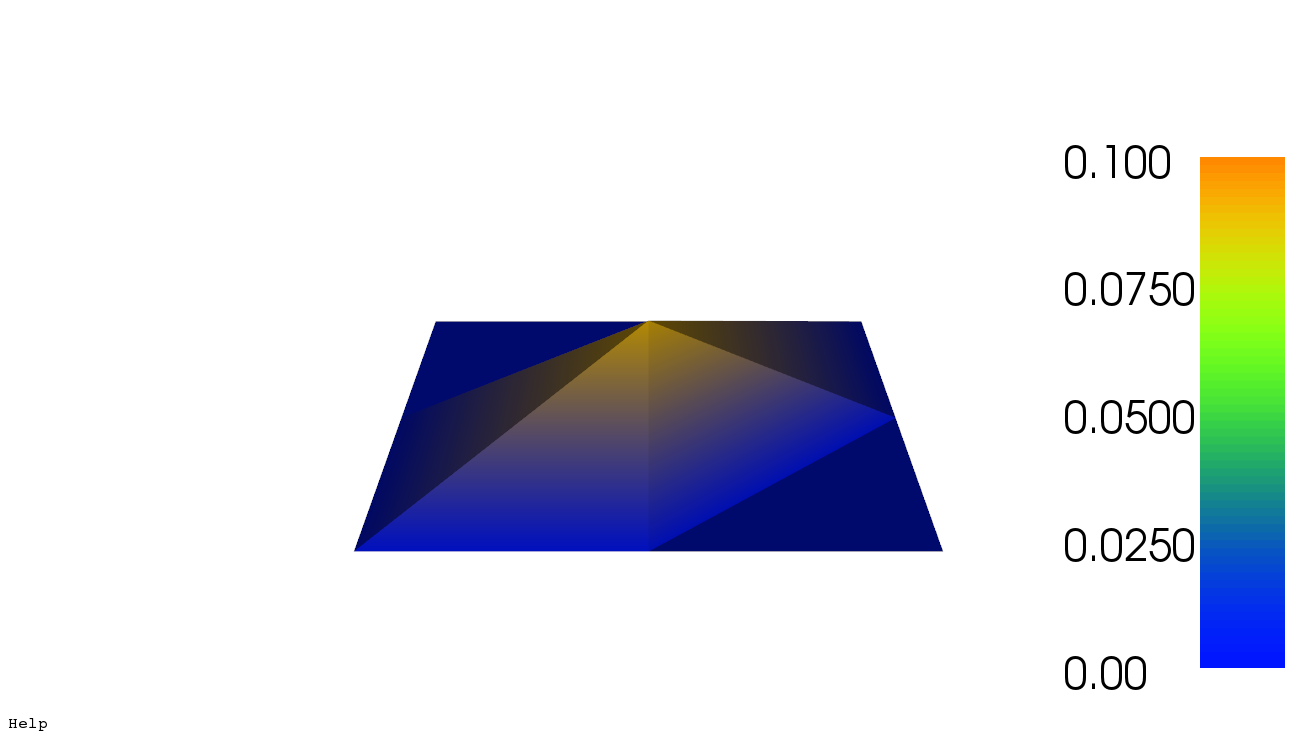
\includegraphics[scale = 0.25]{images/4.png}
	\caption{$2 * 2$ elements}
\end{figure}
Order of convergence data
\begin{lstlisting}
Max error in Run 1 is 0.05900472985458862785
Max error in Run 2 is 0.02119882894487590264
Max error in Run 3 is 0.00550957587228301238
Max error in Run 4 is 0.00110141248956971416
Max error in Run 5 is 0.00005668741721423509
Order of convergence
1.47684603606
1.94397140098
2.32258639099
4.2801825243
\end{lstlisting}
\begin{figure}[h]
	\center
	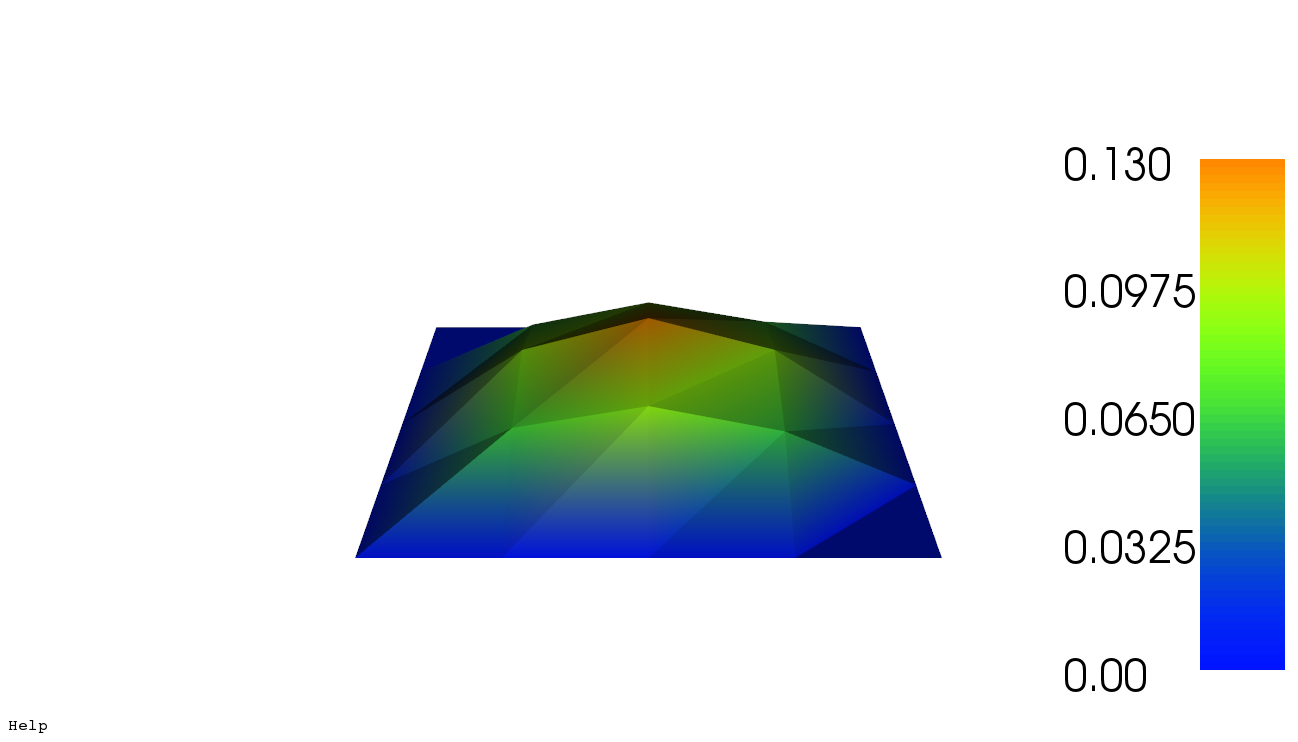
\includegraphics[scale = 0.25]{images/16.png}
	\caption{$4 * 4$ elements}
\end{figure}
\begin{figure}[h]
	\center
	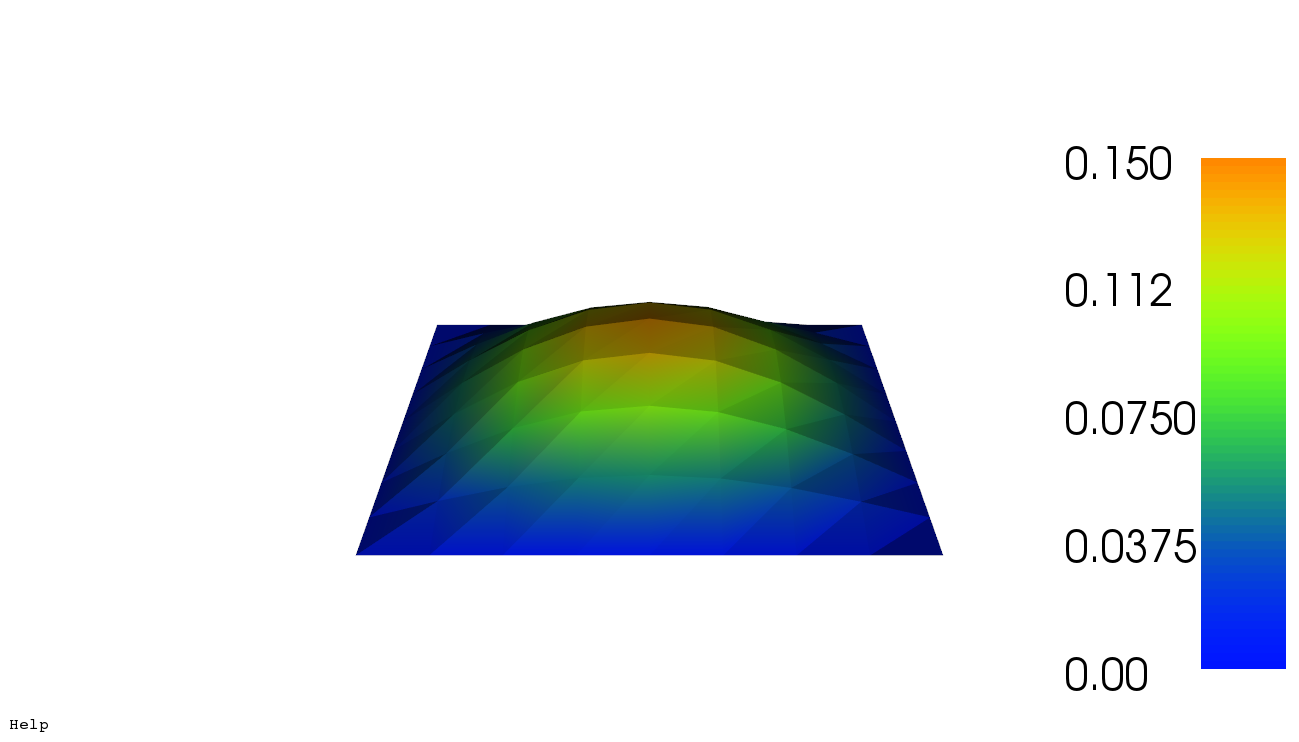
\includegraphics[scale = 0.25]{images/64.png}
	\caption{$8 * 8$ elements}
\end{figure}
\begin{figure}[h]
	\center
	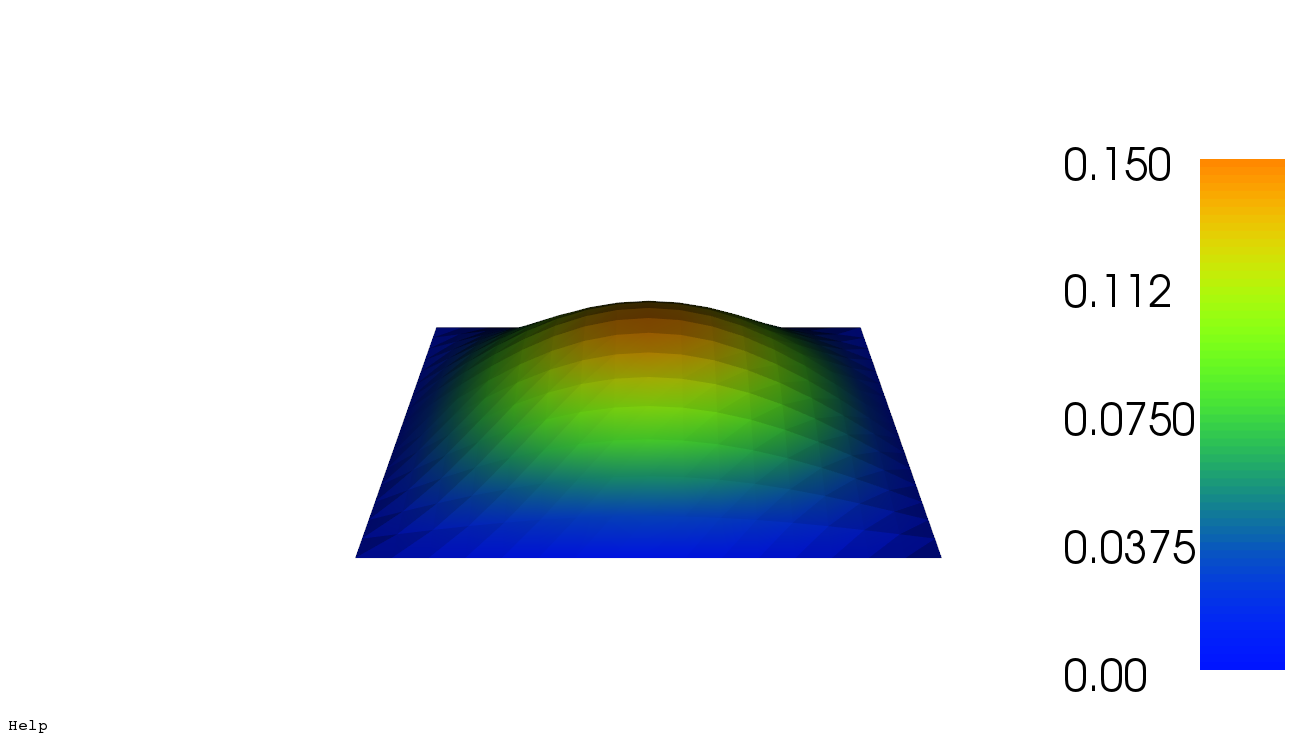
\includegraphics[scale = 0.25]{images/256.png}
	\caption{$16 * 16$ elements}
\end{figure}
\begin{figure}[h]
	\center
	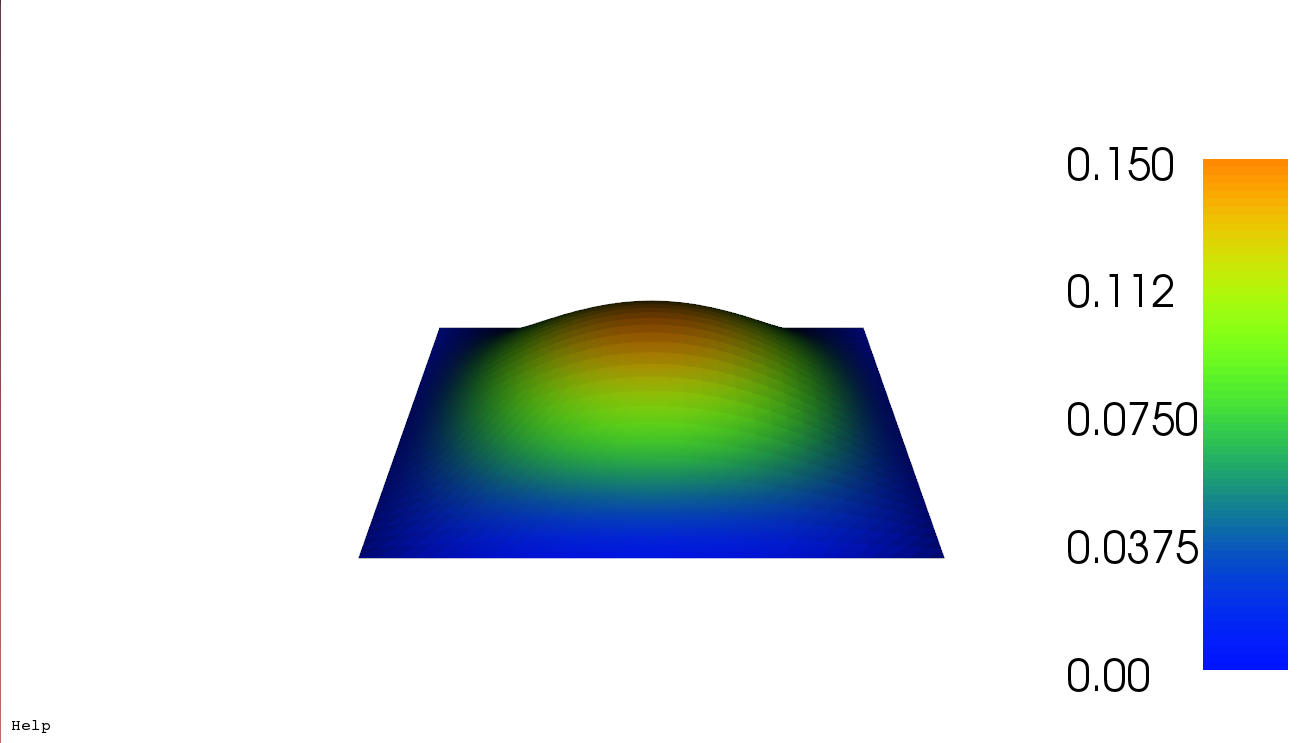
\includegraphics[scale = 0.25]{images/1024.png}
	\caption{$32 * 32$ elements}
\end{figure}